\begin{figure}
        \centering
        \begin{subfigure}[b]{0.75\textwidth}
                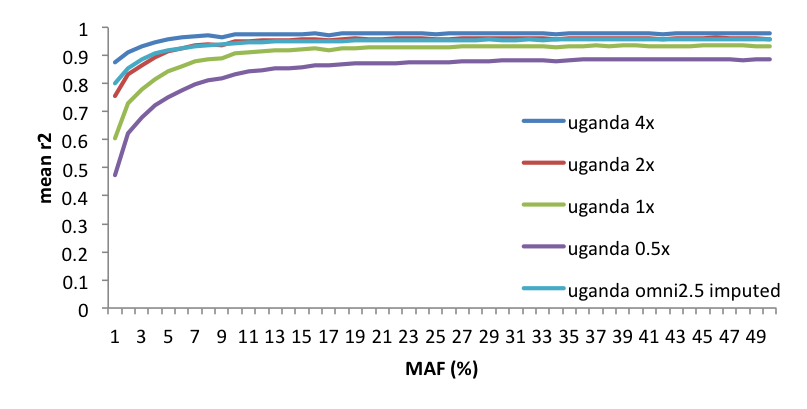
\includegraphics[width=\textwidth]{fig/SN12f5a}
                \caption{Uganda}
                \label{fig:SN12f5uganda}
        \end{subfigure}%

        \begin{subfigure}[b]{0.75\textwidth}
                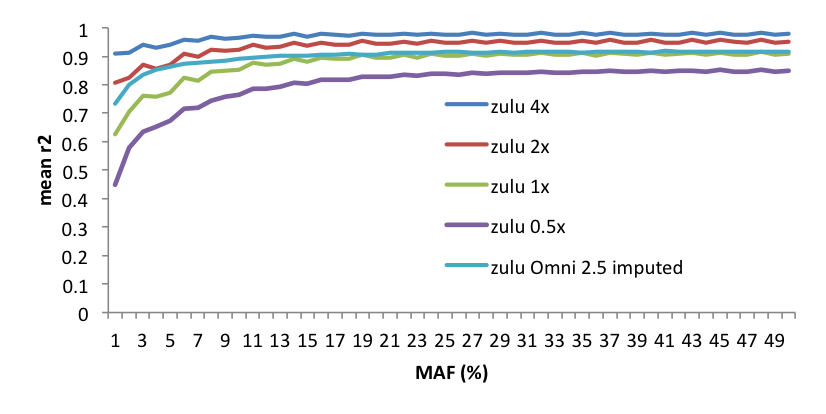
\includegraphics[width=\textwidth]{fig/SN12f5b}
                \caption{Zulu}
                \label{fig:zulu}
        \end{subfigure}

        \begin{subfigure}[b]{0.75\textwidth}
                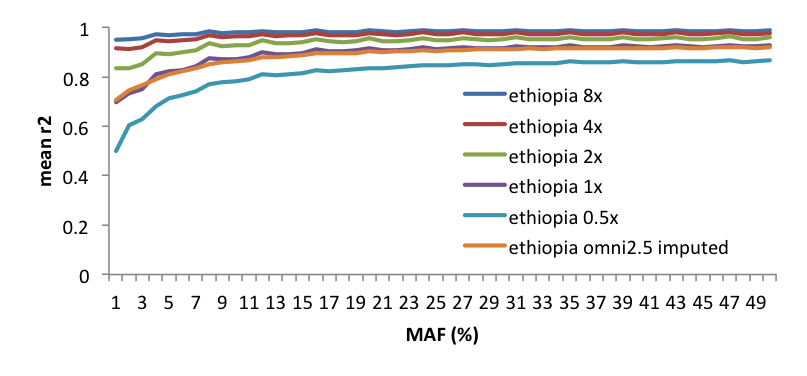
\includegraphics[width=\textwidth]{fig/SN12f5c}
                \caption{Ethiopia}
                \label{fig:ethiopia}
        \end{subfigure}
        \caption[Correlation with imputed chip data and sequence data after downsampling to lower coverage.]{Correlations between different designs and overlapping genotype data from the Omni 2.5M array for each of the 3 populations; Uganda (top), Zulu (middle) and Ethiopia (bottom). The line labelled "Omni 2.5M imputed" for each design represents the correlation between data imputed from the Omni 2.5M array using the \gls{1000G} phase 1 v3 integrated panel, and the original data genotyped on the chip array.}
        \label{fig:SN12f5}
\end{figure}